\documentclass[12pt, aspectratio=169]{beamer}
\usefonttheme{serif}
\usepackage{multicol}
\usepackage{minted}
\usepackage{amsmath}
\usepackage{amsfonts}
\usepackage{amssymb}
\usepackage{graphicx}
\usepackage{tabularx}
\usepackage{braket}
\usepackage[utf8]{inputenc}
\usepackage[numbers]{natbib} 
\author[Debanjan Kola \& Nishanka Das]{%
Debanjan Kola \& Nishanka Das\\
\small Ramakrishna Mission Vivekananda Centenary College, Rahara\\[1ex]
\small \textit{Supervised by: Prof.  Amlan Chakrabarti}\\
A.K. Choudhury School of Information Technology, University of Calcutta
}
\date{\today}

\title{Simulation and Analysis of Quantum Algorithms through GPU Computing}
%\setbeamercovered{transparent} 
%\setbeamertemplate{navigation symbols}{} 
%\logo{} 
%\institute{} 
%\subject{hi} 

\definecolor{myblue}{RGB}{0,102,204} 

\usetheme{Madrid}
\usecolortheme[named=myblue]{structure} 

\begin{document}

\begin{frame}
\titlepage{}
\end{frame}
\begin{frame}[allowframebreaks]{Contents}
    \tableofcontents
\end{frame}

\section{Introduction}
\begin{frame}{Introduction}
 \begin{block}{The Evolution of Computational Power: From Classical to Quantum Computing}
 Why Did We \textbf{Start Thinking} About Quantum Computers?  According to \textbf{Moore’s Law} , the number of transistors in an integrated circuit (IC) doubles approximately every two years. This means the size of individual transistors on a
chip has been steadily decreasing from around $20 \mu m$  in 1968 to just 3 nm 
 in 2022.     
 \end{block}

\end{frame}

\begin{frame}{Moore’s Law}
\begin{figure}
    \centering
    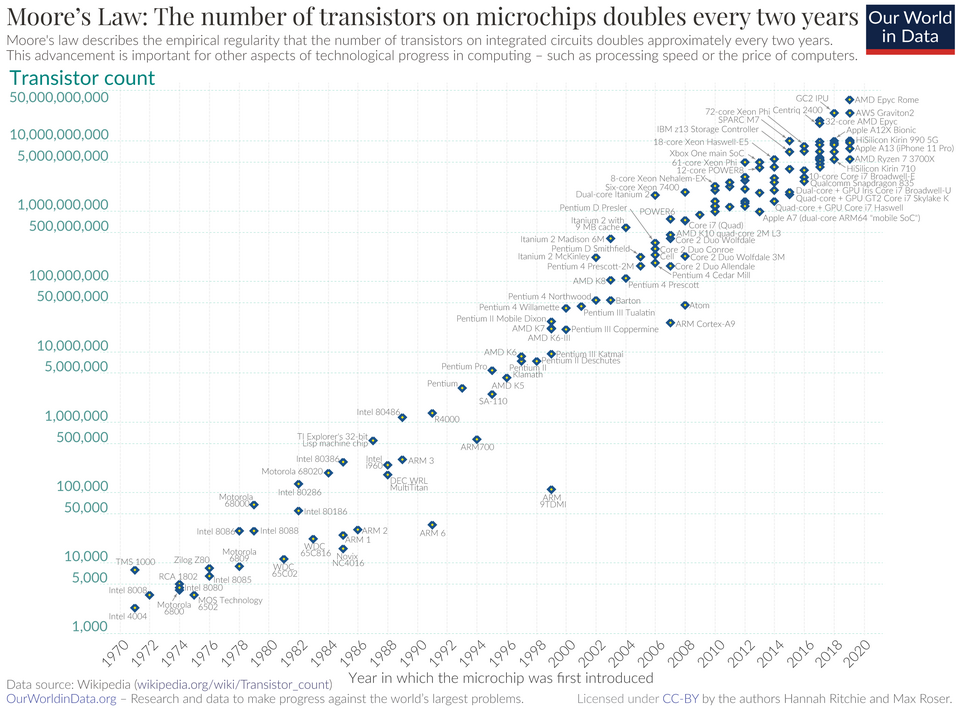
\includegraphics[width=0.6\linewidth]{11.png}
%    \caption{Moore’s Law}
    \label{fig:moore}

\end{figure}
\end{frame}
\begin{frame}{Many-Worlds Interpretation and Quantum Possibilities}
In 1957, \textbf{Hugh Everett} proposed the \textit{Many-Worlds Interpretation (MWI)} of quantum mechanics. 

\vspace{1em}

According to this theory, we inhabit only a small slice of physical reality, and the totality of all quantum possibilities forms what is called the \textbf{multiverse}.

\vspace{1em}

For example, the hydrogen wave function is a mathematical expression that describes the \textbf{probability amplitude} of finding an electron in a specific state and position within a hydrogen atom. 

\vspace{1em}

It reflects the fundamental principles of quantum mechanics, highlighting the probabilistic nature of quantum states.
\end{frame}
\begin{frame}{Hydrogen Atom Wave Function }
\begin{figure}
    \centering
    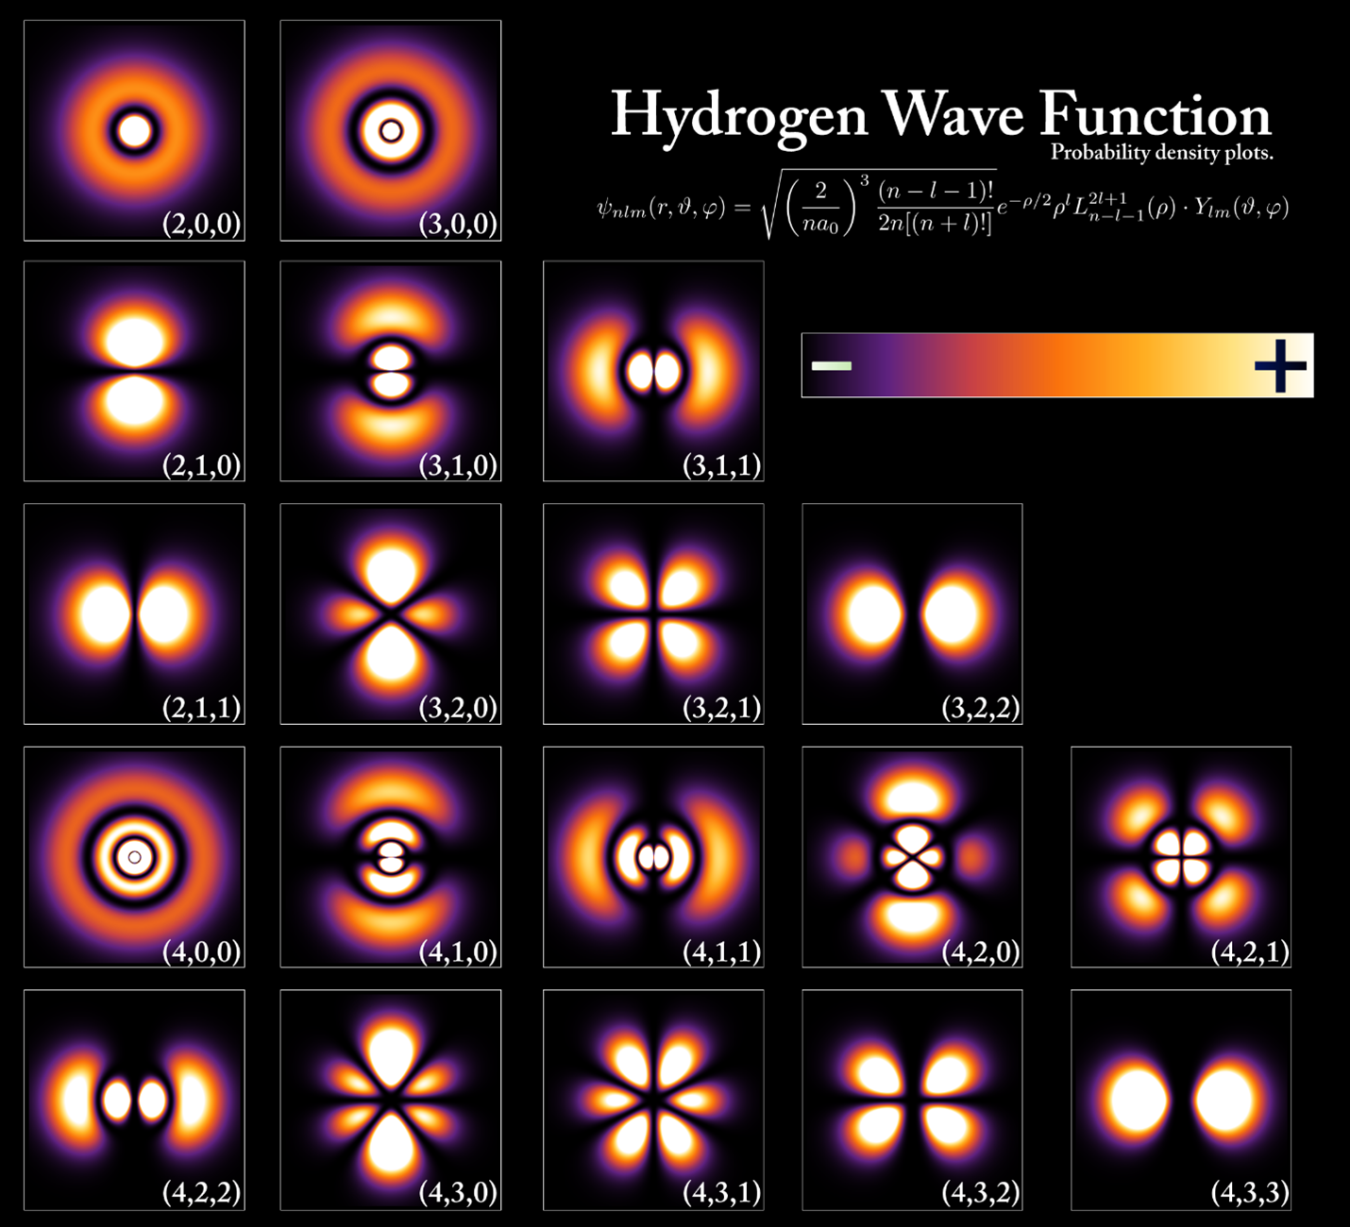
\includegraphics[width=0.4\linewidth]{12.png}
%    \caption{Hydrogen Atom Wave Function}
    \label{fig:enter-label}
\end{figure}
\tiny\textit{Source: Forinash, Kyle. Hydrogen W Simulation. Indiana University Southeast.}
\end{frame} 
\begin{frame}{Observables and the Multiverse Perspective}
In classical physics, a point particle has three degrees of freedom, corresponding to the three real numbers required to specify its position in space: \textit{(x, y, z)}.

\vspace{1em}
\begin{figure}
    \centering
    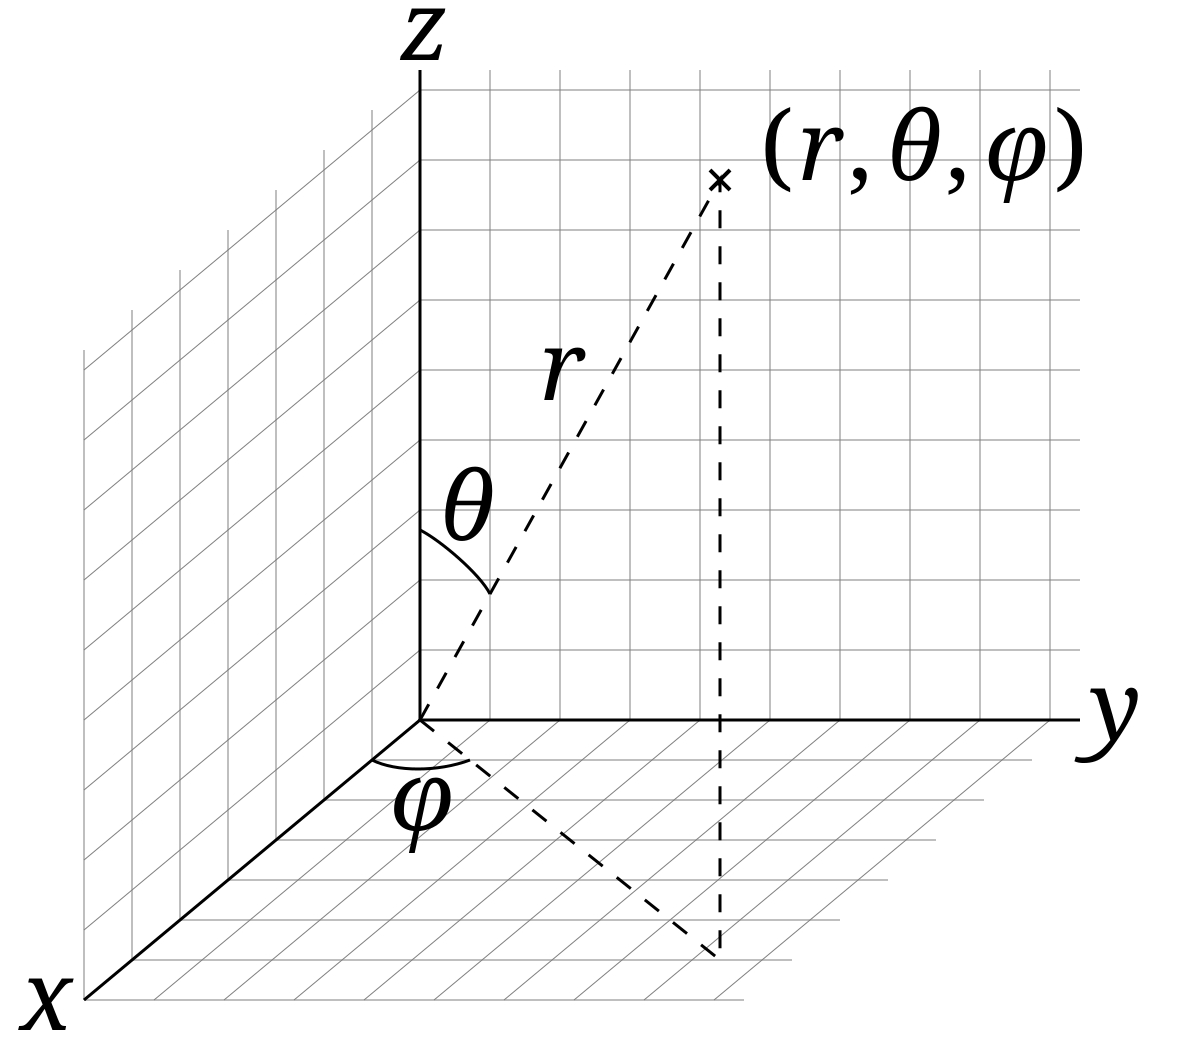
\includegraphics[width=0.3\linewidth]{13.png}
    \caption{Degrees of Freedom}
    \label{fig:enter-label}
\end{figure}
\end{frame}
\begin{frame}{Spectrum of Observables and Quantum Phenomena}
However, in quantum physics, we refer to \textbf{observables}, which represent not only what we measure in our universe, but also values of corresponding measurements across other universes in the \textit{multiverse}.

Consider a compass: the angle between its two arms might be 37° in one universe. This angle is represented as $\hat{\theta}(t)$, an observable that varies with time.

\vspace{1em}

The \textbf{spectrum} of this observable is the set of all possible angles between the arms across all universes—capturing the multiverse structure of quantum reality.
\end{frame}

\begin{frame}{Quantum Superposition}

\vspace{0.5em}

Two of the most profound and non-classical phenomena in quantum mechanics are:
Entanglement and Superposition .\\

\textbf{Superposition :}\\

In classical computing, a bit can exist in one of two states: 0 or 1. In contrast, a qubit, the basic unit of quantum information, can exist in a superposition of both 0 and 1 simultaneously. Mathematically, this is represented as:

\[
|\psi\rangle = \alpha|0\rangle + \beta|1\rangle,
\]

where \(\alpha\) and \(\beta\) are complex probability amplitudes, and \(|\alpha|^2 + |\beta|^2 = 1\).
\end{frame}
\begin{frame}{Quantum Entanglement}
This means a single qubit can represent multiple states at once, and with \(n\) qubits, a quantum computer can represent \(2^n\) states in parallel. This exponential scaling of representational capability is behind the vast parallelism of quantum computation.\\


\textbf{Entanglement:} Entanglement is a quantum phenomenon where the state of one qubit becomes intrinsically linked to the state of another, regardless of the distance separating them. An entangled pair of qubits cannot be described independently; the state of the entire system must be considered.

For example, in an entangled Bell state:

\[
|\Phi^+\rangle = \frac{1}{\sqrt{2}} (|00\rangle + |11\rangle),
\]
\end{frame}
\begin{frame}{Superposition and Entanglement}
measuring one qubit simultaneously determines the state of the other. This allows for correlated operations and information sharing across qubits in ways that classical systems cannot replicate.
\begin{figure}
    \centering
    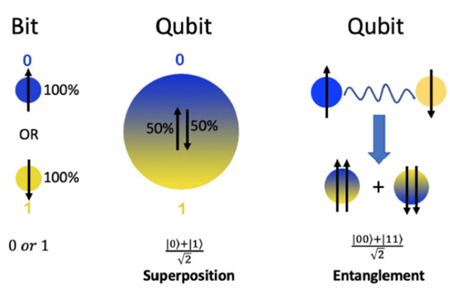
\includegraphics[width=0.5\linewidth]{14.png}
 %   \caption{Superposition and Entanglement}
    \label{fig:label}
\end{figure}
\end{frame}



   


%\begin{frame}{Contents}
%    \begin{itemize}
%        \item Introduction to Quantum Computation by DK
%        \item Evolution and Simulation of Quantum Computation by ND
%        \item Usability of Quantum Support Vector Machines in Quantum %Finance by DK
%        \item An Hybrid approach to words Quantum Neural Networks by ND
%       \item Conclusion by DK
%    \end{itemize}
%\end{frame}
\section{Evolution and Simulation of Quantum Computation}
\begin{frame}{Evolution and Simulation of Quantum Computation}
    \begin{itemize}
        \item Evolution of Quantum Computers
        \item Evolution of Quantum Hardware
        \item Why does Quantum Computing needs to be simulated?
        \item Tools for simulating Quantum Computers
        \item Why CUDA-Quantum ?
        \item Snippet of CUDA-Quantum
        \item Result Comparison of CUDA-Quantum and Real Quantum Computer
        \item Limitations of CUDA-Quantum
        \item Bridging CUDA-Q and Qiskit
        \item Methodology 
        \item Usage and Further Development
    \end{itemize}
\end{frame}
\begin{frame}{Evolution of Quantum Computers }
\begin{figure}
    \centering
    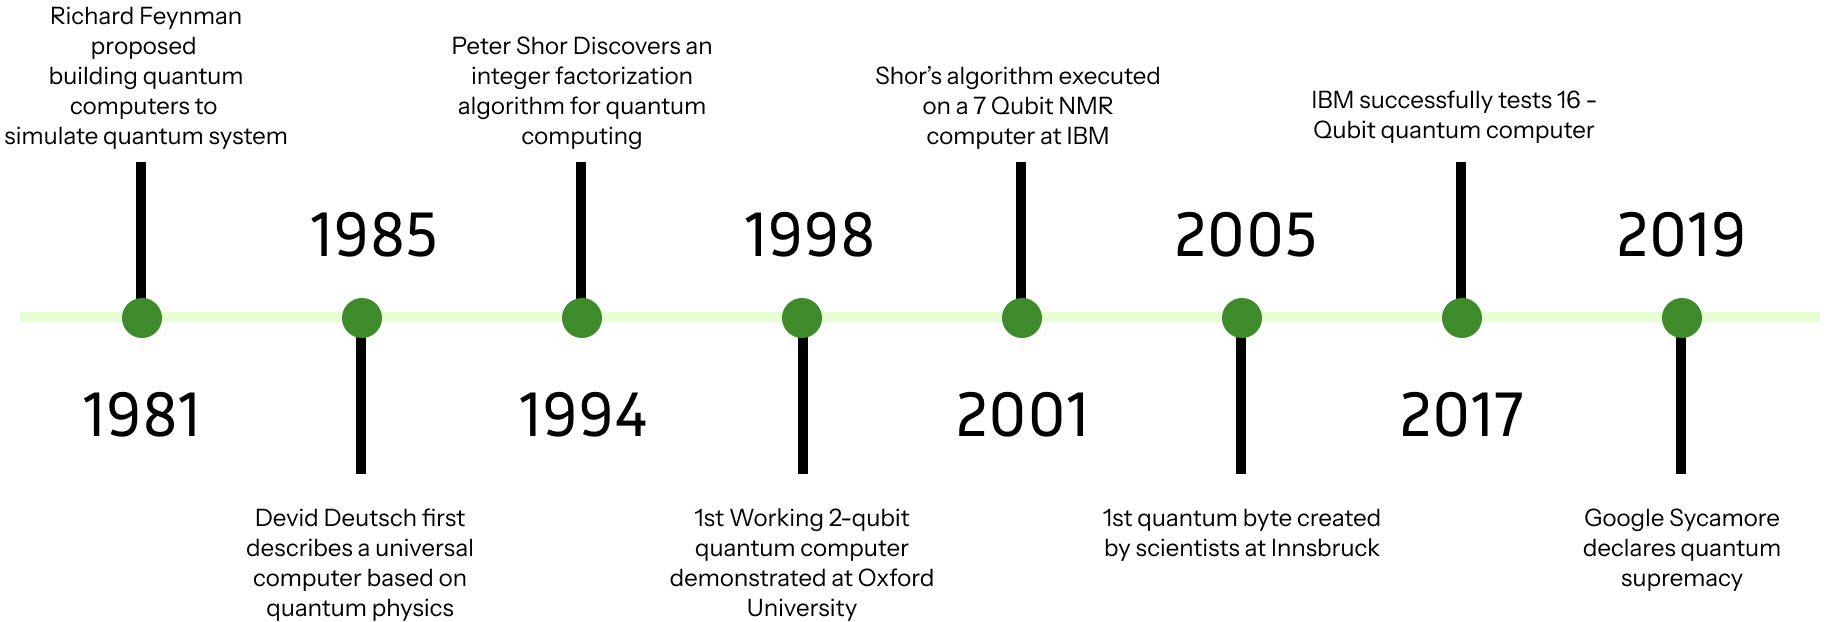
\includegraphics[width=0.9\linewidth]{evaluation.png}
    \caption{From papers to hardware}
    \label{fig:enter-label}
\end{figure}
\hspace{1cm}
\tiny\textit{Source: Indiana University, ScienceNode }
\end{frame}
\begin{frame}{Evolution of Quantum Computers (HW) }
\begin{figure}
    \centering
    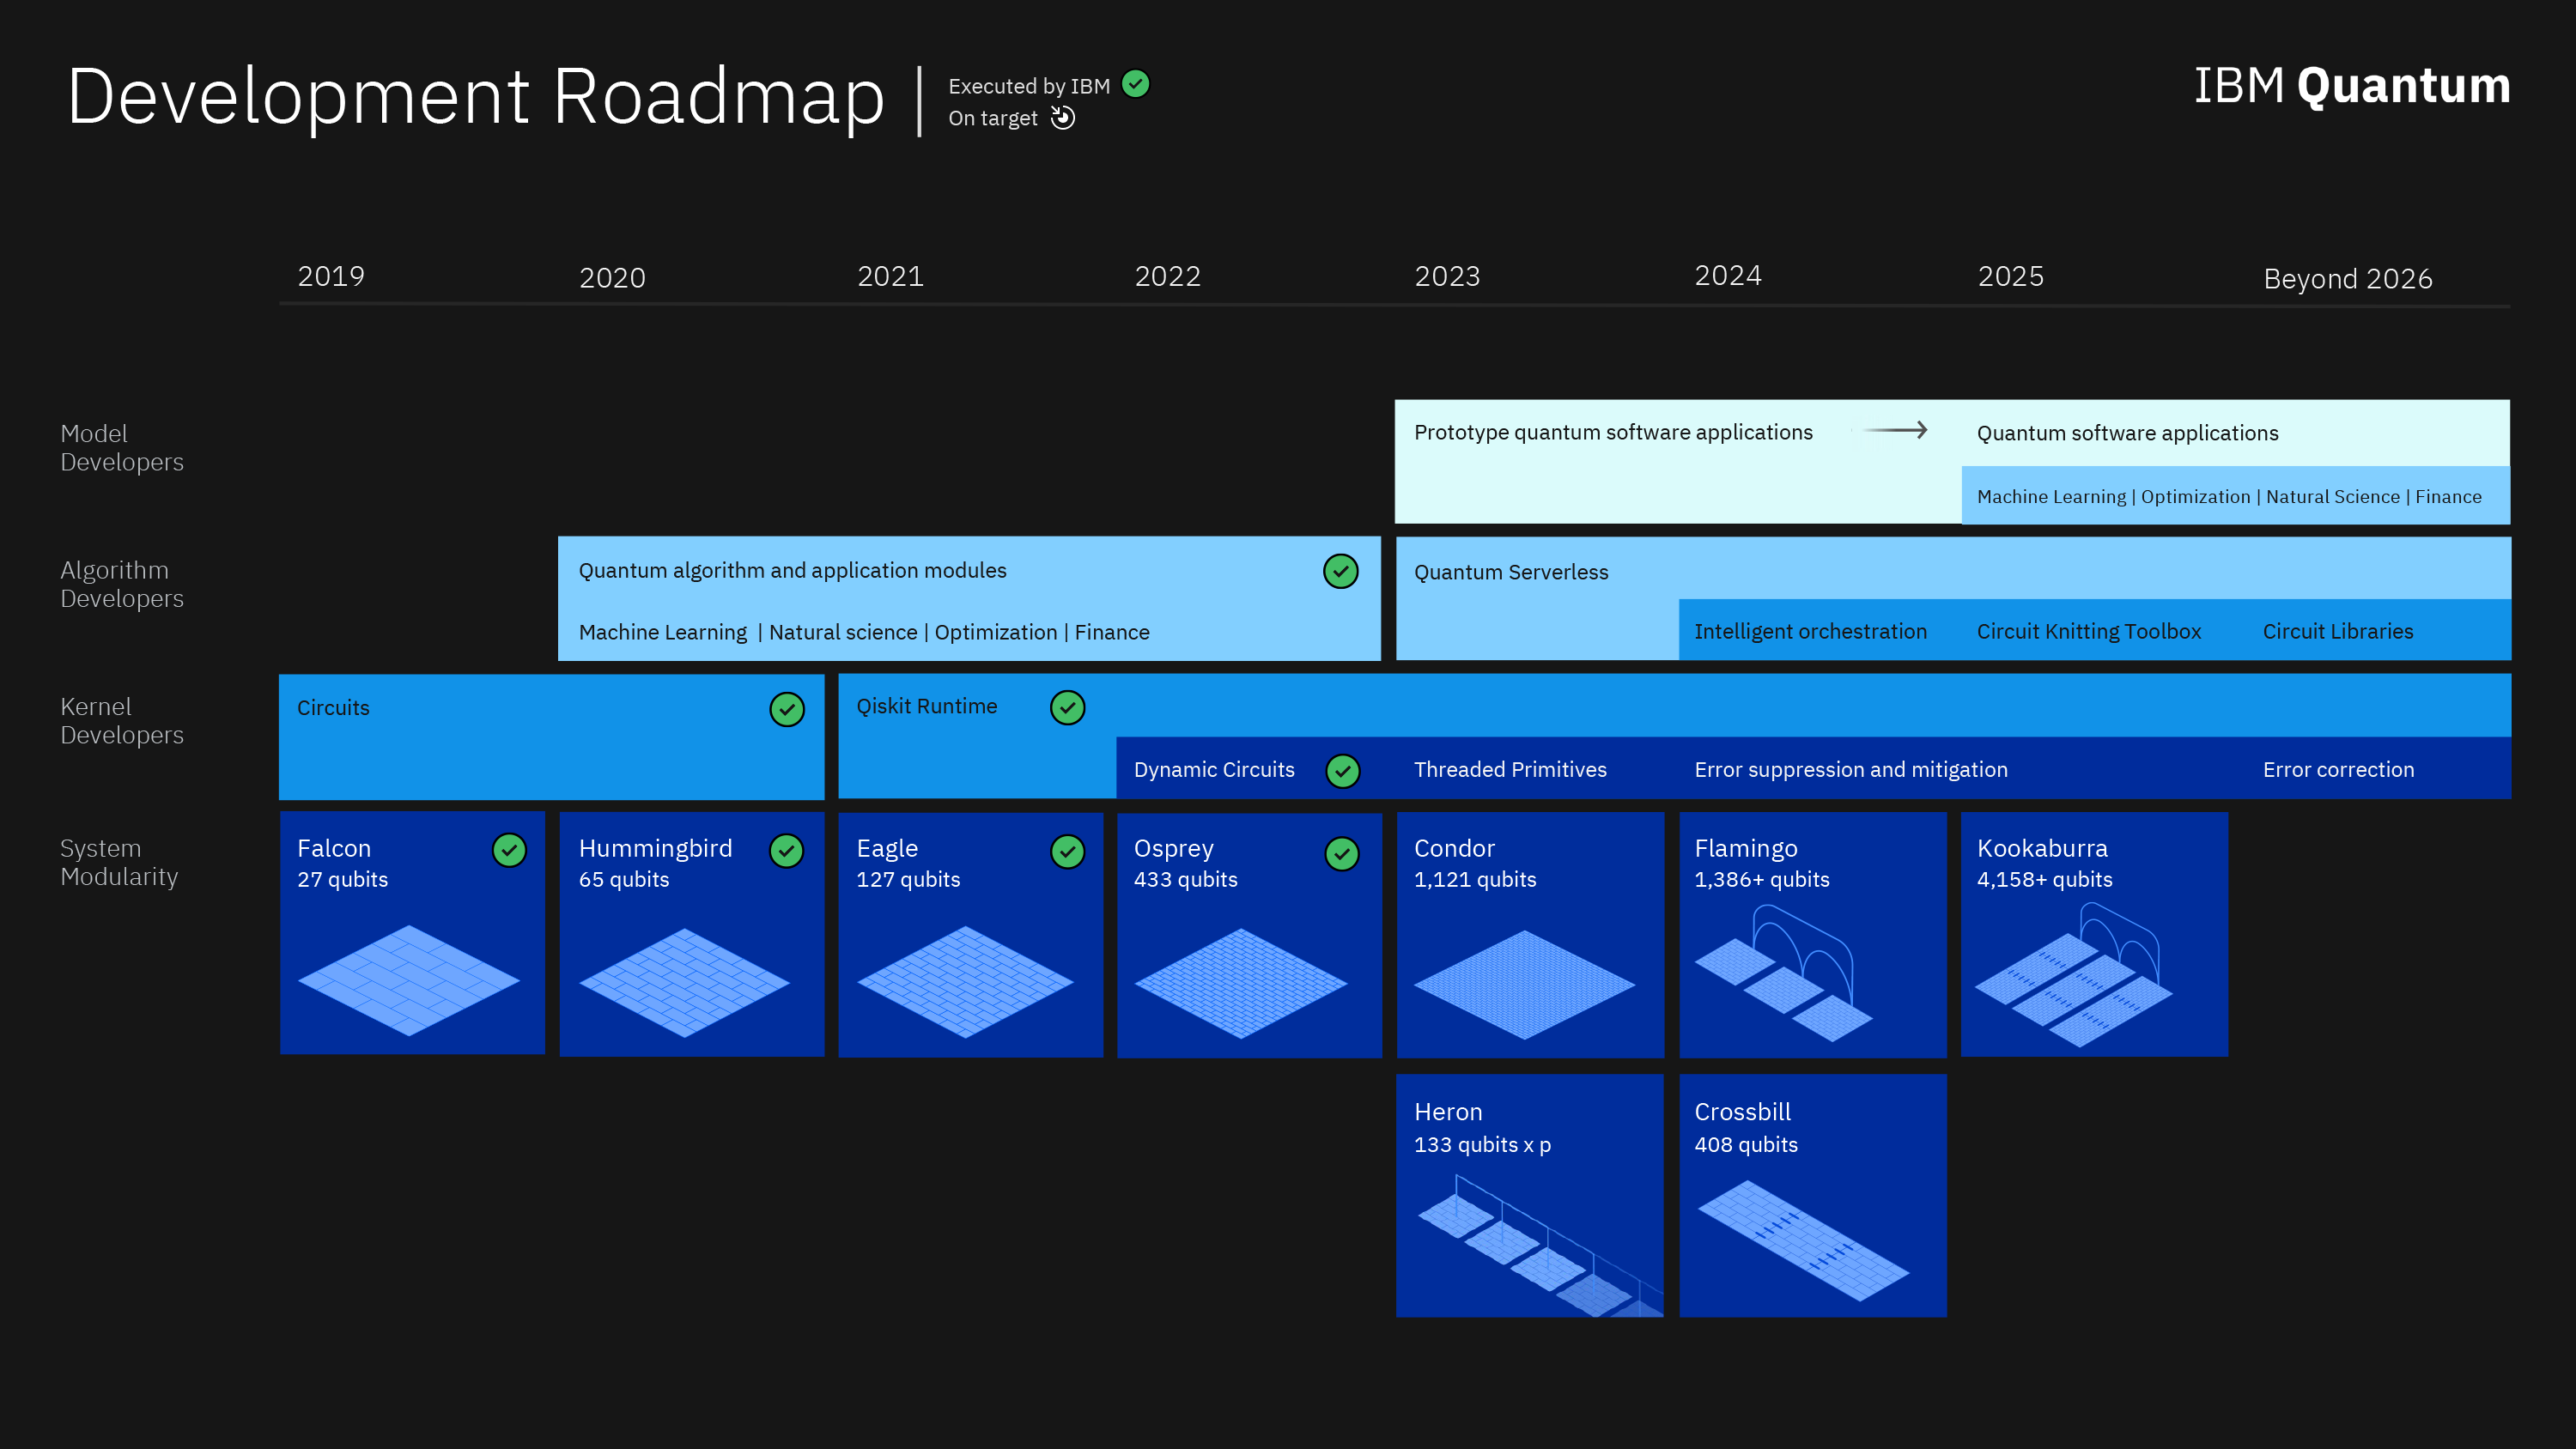
\includegraphics[width=0.75\linewidth]{rodemap-ibm.png}
    \caption{IBM Road Map}
    \label{fig:enter-label}
\end{figure}
\hspace{1cm}
\tiny\textit{Source: newsroom.ibm.com}
\end{frame}
\section{Why does Quantum Computing need to be simulated?}
\begin{frame}{Why does Quantum Computing need to be simulated?}
\begin{itemize}
    \item \textbf{NISQ Era Challenges :}  Current quantum computers are in the Noisy Intermediate-Scale Quantum (NISQ) era, meaning they have limited qubits and high error rates. Simulators help test and refine quantum algorithms before real execution.
    \item  \textbf{Algorithm Development :} Simulators allow researchers to design, debug, and optimize quantum programs before running them on actual hardware.
    \item \textbf{Performance Benchmarking :} Comparing simulated vs. real hardware results helps improve error correction techniques and optimize quantum gates.
\end{itemize}
\end{frame}

\begin{frame}{Tools for simulating Quantum Computers}
\begin{figure}
    \centering
    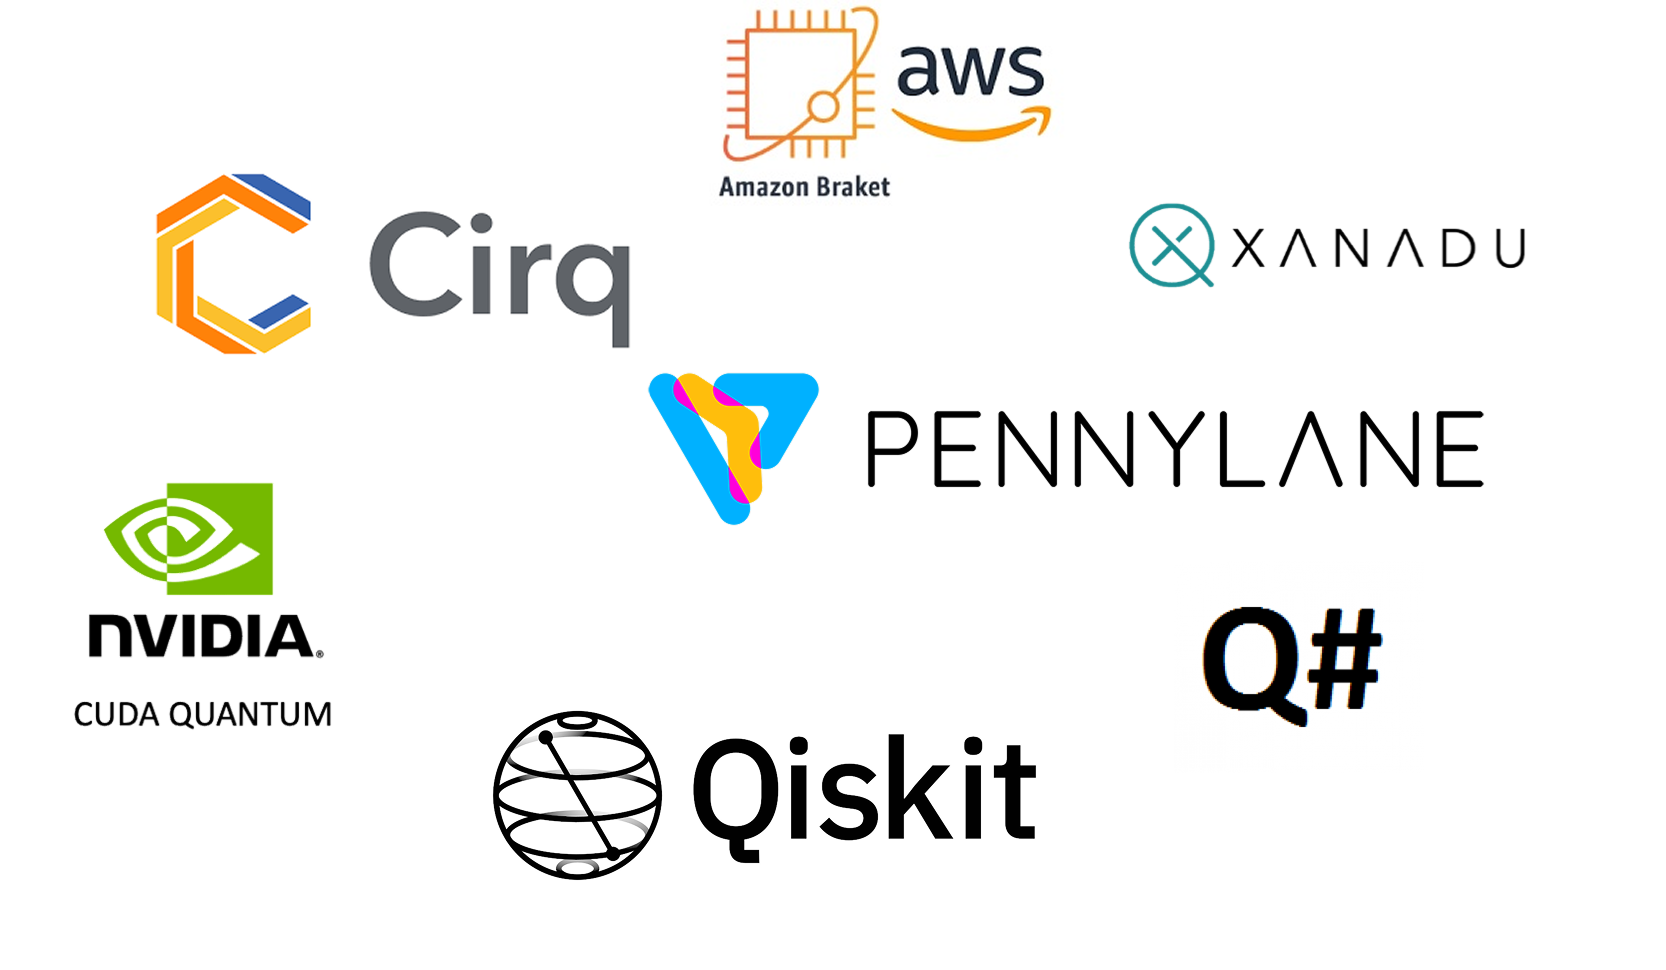
\includegraphics[width=0.8\linewidth]{quan_programminglang.png}
  
    \label{fig:enter-label}
\end{figure}
\end{frame}
\section{CUDA-Quantum}
\begin{frame}{Why CUDA-Quantum ?}
\begin{figure}
    \centering
    \includegraphics[width=1\linewidth]{backends.png}
\end{figure}
\end{frame}


\begin{frame}[fragile]{Snippet of CUDA-Quantum}
\scriptsize
\begin{minted}{python}
@cudaq.kernel
def kernel_to_draw():
    q = cudaq.qvector(4)
    h(q)
    x.ctrl(q[0], q[1])
    y.ctrl([q[0], q[1]], q[2])
    z(q[2])
    swap(q[0], q[1])
    swap(q[0], q[3])
    swap(q[1], q[2])
    r1(3.14159, q[0])
    tdg(q[1])
    s(q[2])
print(cudaq.draw(kernel_to_draw))
\end{minted}
\begin{figure}
    \centering
    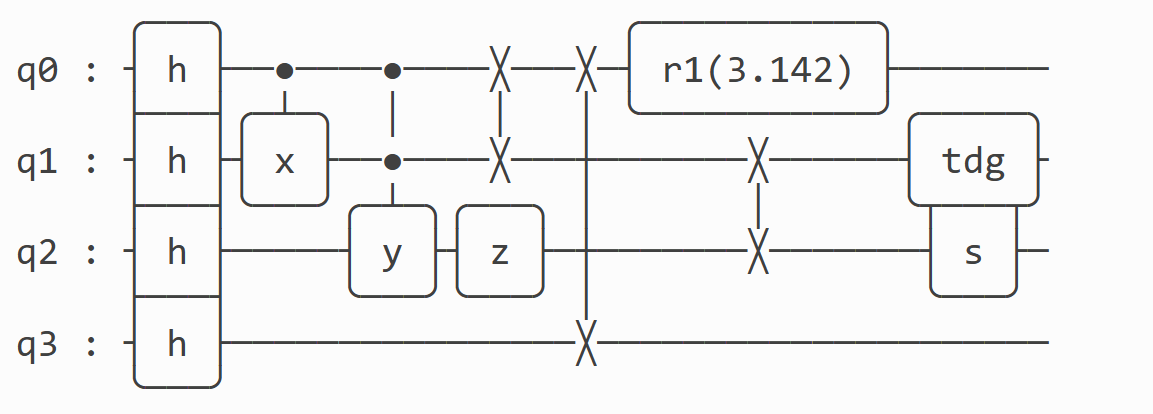
\includegraphics[width=0.4\linewidth]{snipp.png}
\end{figure}
\end{frame}


\begin{frame}{Result Comparison of CUDA-Quantum and Real Quantum Computer }
    \begin{figure}
        \centering
        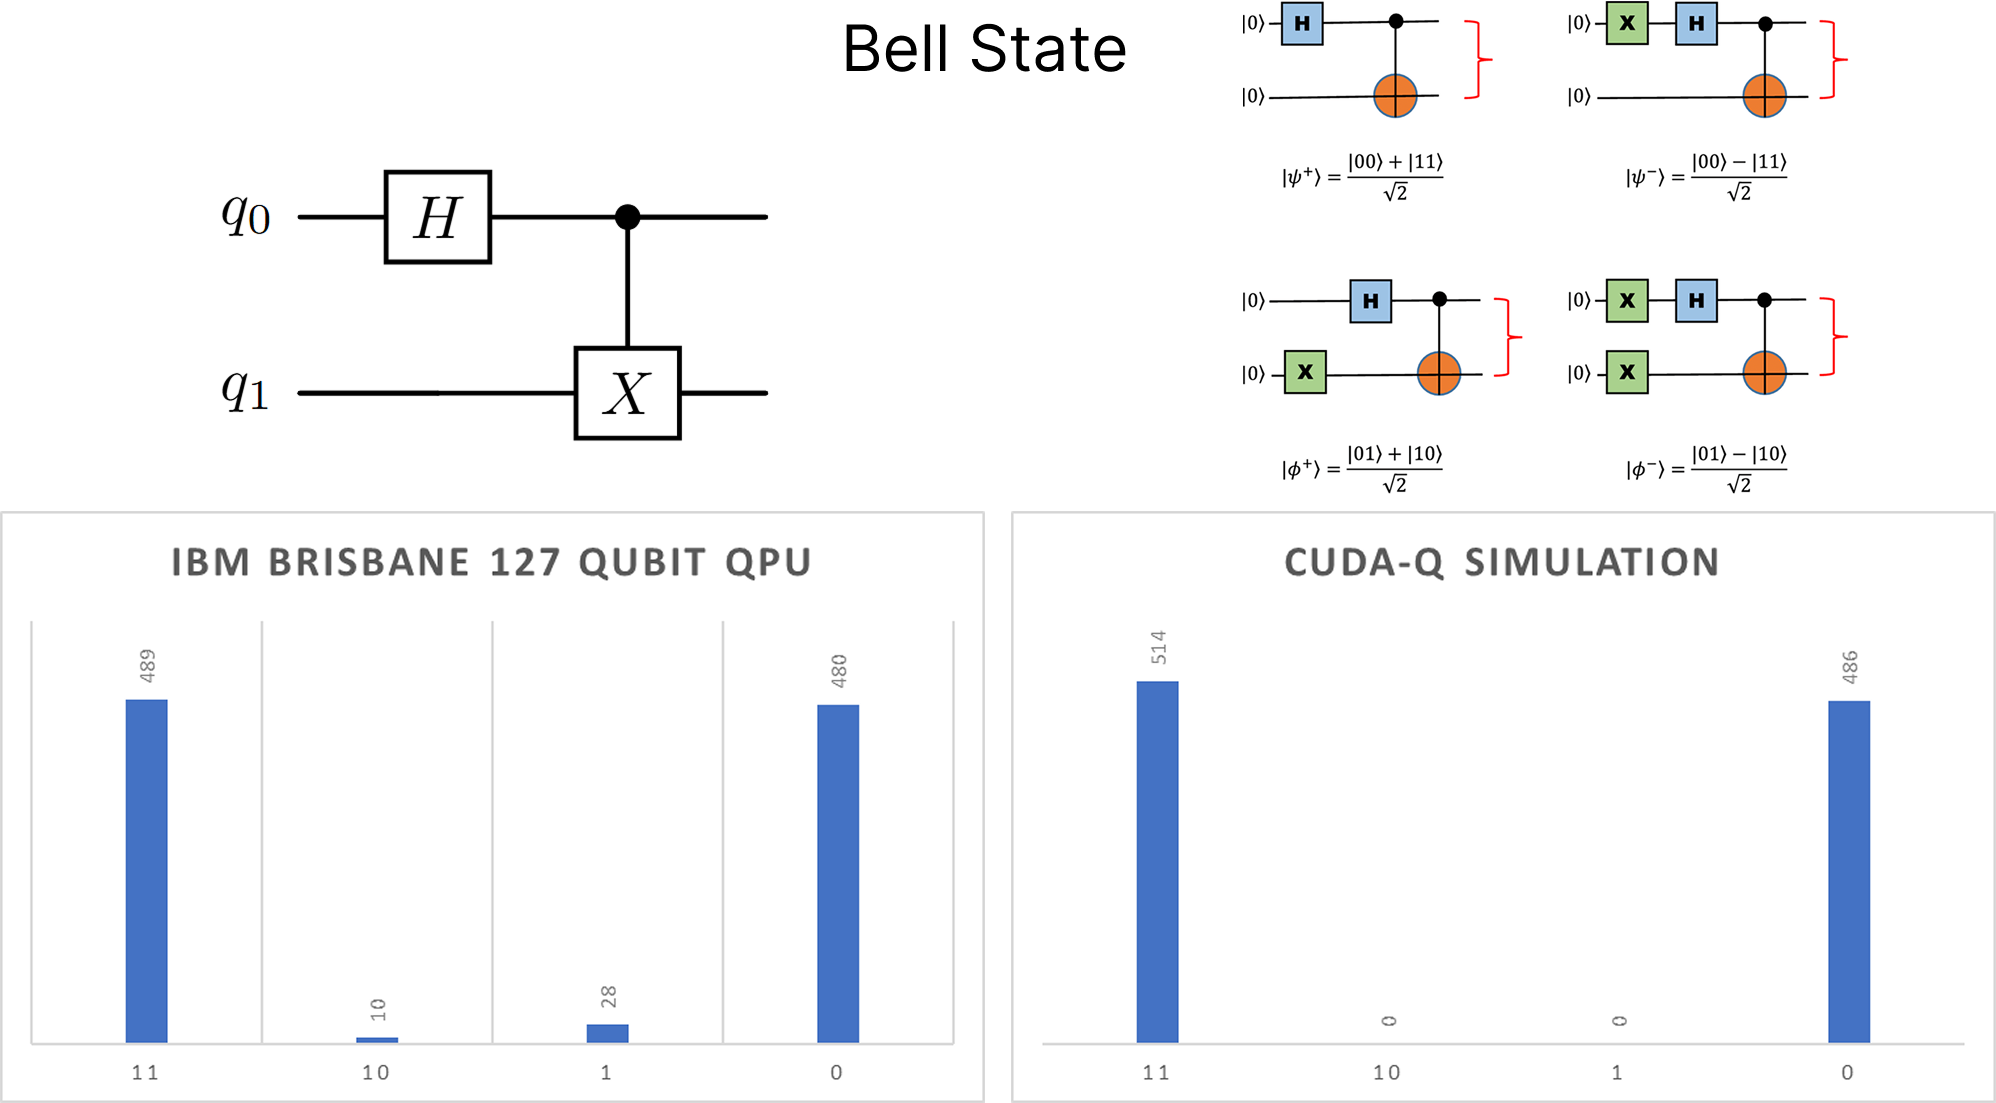
\includegraphics[width=0.7\linewidth]{bell.png}
    \end{figure}
\end{frame}


\begin{frame}{Limitations of CUDA-Quantum}
\begin{itemize}
    \item Cuda Quantum offers GPU simulation that is able to simulate upto 45+ qubits even with the highest power GPUs. The following table describes how much memory is need to simulate for how many qubits.
    \vspace{.5cm}\\
    \begin{tabularx}{0.8\textwidth} { 
  | >{\centering\arraybackslash}X 
  | >{\centering\arraybackslash}X |}
 \hline
10 qubit & 8 KB\\
 \hline
20 qubit & 8 MB\\
\hline
40 qubit & 8 GB\\
\hline
60 qubit & 8192 PB\\
\hline
\end{tabularx}
\end{itemize}
\end{frame}

\begin{frame}{Bridging CUDA-Quantum and Qiskit}
\begin{itemize}
    \item Why Qiskit?\\
    Qiskit offers free 10 minutes access of IBM Quantum Computer per month to any user. 
    \item We can design large quantum circuits to simulate there result and if they are accurate, we can test them on original Quantum Computers. 
    \item Parsing with Abstract Syntax Tree (AST): Converts CUDA-Q source code into a structured format.

    \item Extracting operations: Identifies quantum gates, extracts parameters and qubits.

    \item Storing in a list: Saves the extracted operations for further processing
\end{itemize}
\end{frame}



\begin{frame}{Methodology of Code conversion }
\begin{figure}
    \centering
    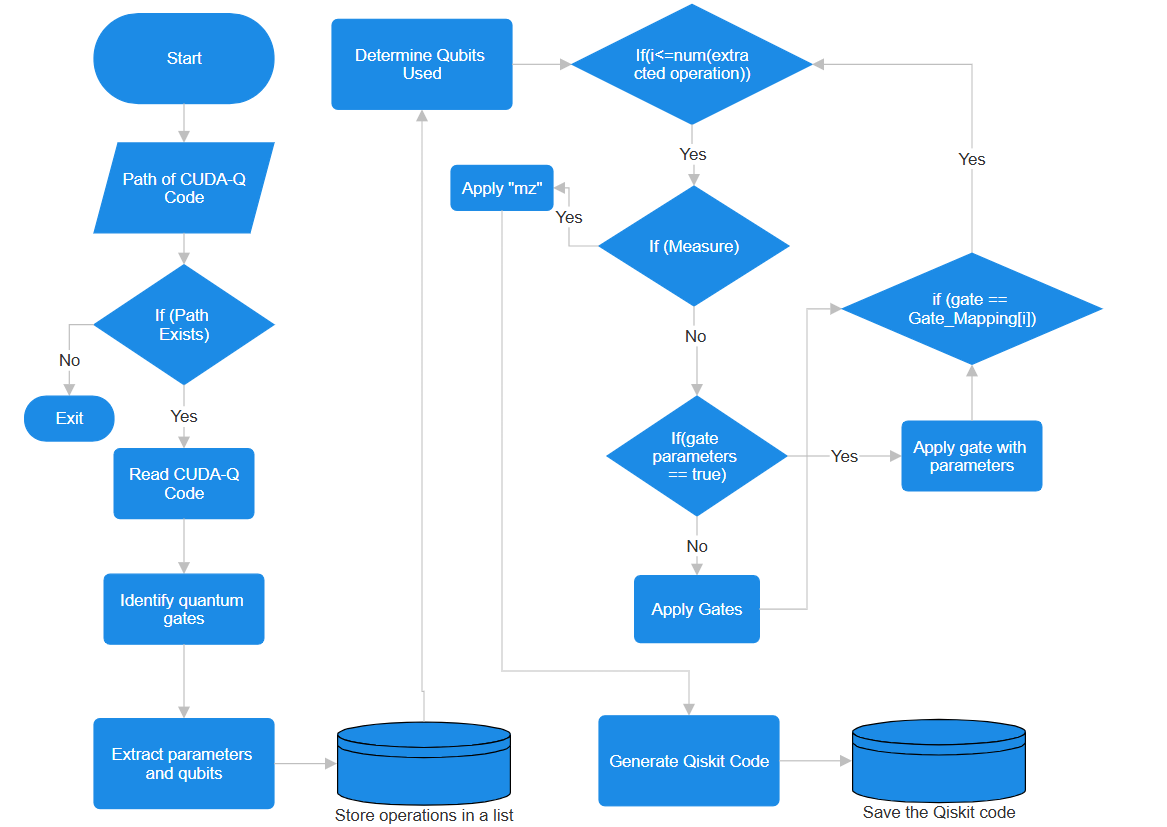
\includegraphics[width=0.6\linewidth]{flow.png}
\end{figure}
\end{frame}


\begin{frame}{Usage and Further Development}
\begin{table}[]
    \centering
    \begin{tabular}{c|c}
      \textbf{CUDA-Q Source Code}   & \textbf{Qiskit Generated Code} \\
       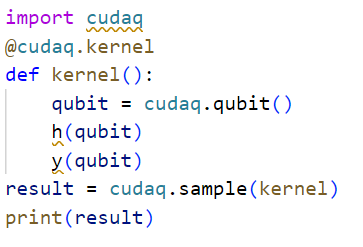
\includegraphics[width = 0.35\linewidth ]{cud.png}  & 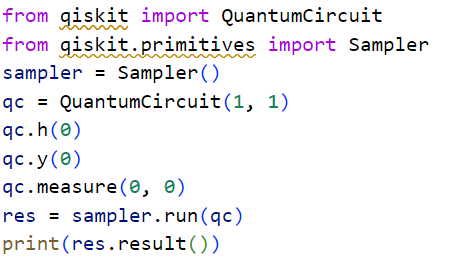
\includegraphics[width = 0.4\linewidth]{qis.png}
    \end{tabular}
\end{table}
\textbf{Future Works}
\begin{itemize}
    \item This Library only includes single-qubit circuit conversions. In further development we can develop a multiqubit conversion library.
\end{itemize}
\end{frame}




\section{Classical SVM vs Quantum SVM}
\begin{frame}{Classical SVM vs Quantum SVM}
This study focuses on the implementation and training of both a classical Support Vector Machine (SVM) and a Quantum Support Vector Machine (QSVM) using an identical credit card transaction dataset.

\vspace{0.5em}

By ensuring consistent input data and evaluation metrics, this comparative analysis aims to assess the performance differences between classical and quantum-enhanced machine learning models.

\vspace{0.5em}

\textbf{Objective:} To explore whether QSVMs can provide improved accuracy in fraud detection and to highlight the potential advantages and limitations of quantum machine learning in solving real-world classification tasks.
\end{frame}
\begin{frame}{Results and Discussion}
    \begin{figure}
    \centering
    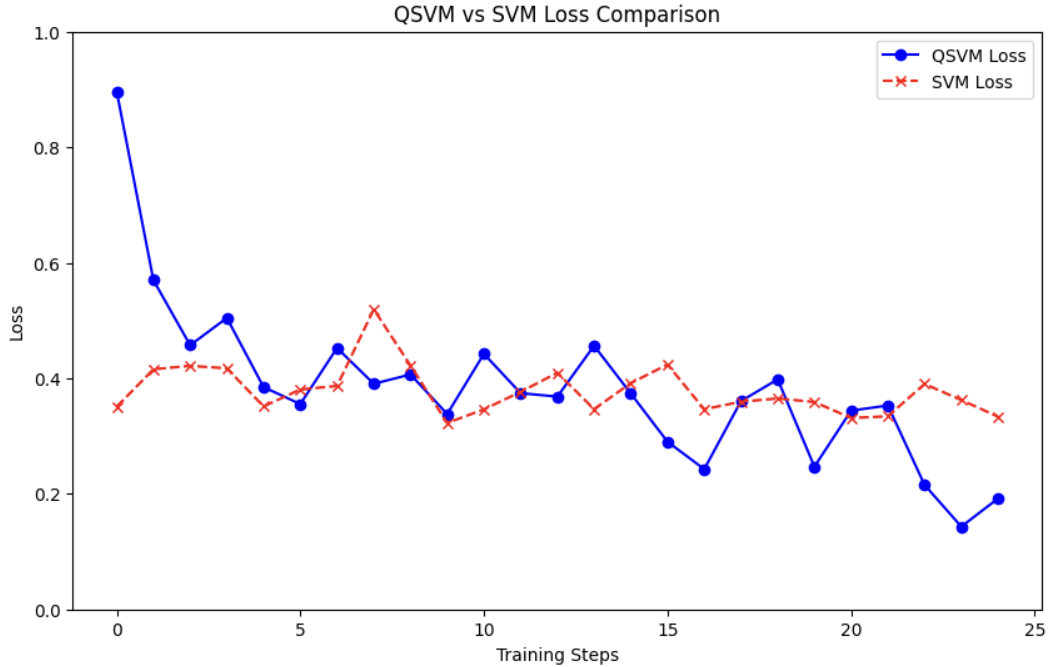
\includegraphics[width=0.4\linewidth]{one.png}
    \caption{QSVM vs. SVM Loss Comparison}
\end{figure}
The graph compares the loss trends of QSVM and SVM over training steps. QSVM
has a steeper initial decline in loss, reflecting faster convergence during training .
\end{frame}
\begin{frame}{Decision Boundary Comparison: QSVM vs Classical SVM}
\begin{figure}
    \centering
    \begin{minipage}{0.48\textwidth}
        \centering
        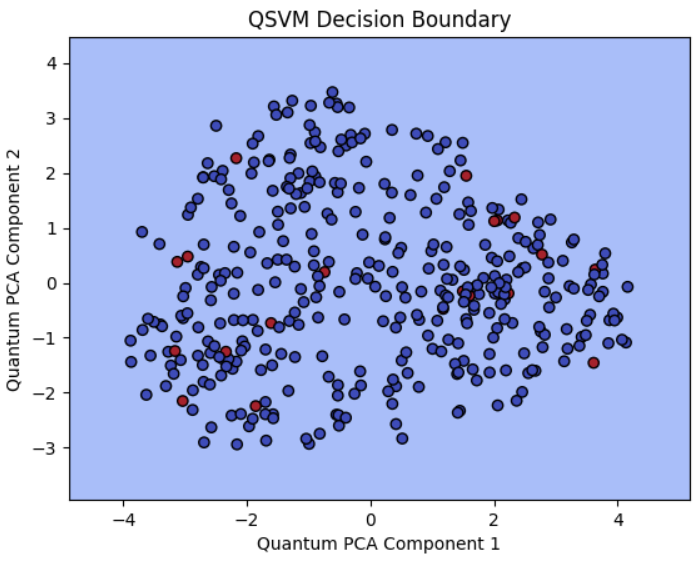
\includegraphics[width=\linewidth]{three.png}
        \textbf{QSVM Decision Boundary}
    \end{minipage} \hfill
    \begin{minipage}{0.48\textwidth}
        \centering
        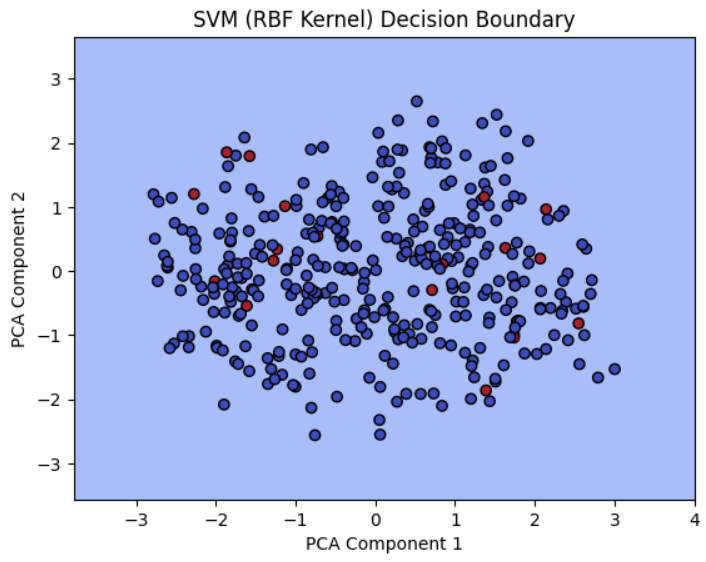
\includegraphics[width=\linewidth]{two.png}
        \textbf{RBF Kernel Decision Boundary (Classical SVM)}
    \end{minipage}
\end{figure}
\end{frame}
\begin{frame}
\begin{block}{Observation}
\textbf{QSVM boundary} correctly distinguishes points in the quantum-transformed feature space; classification regions are indicated in the background as blue. Blue and red dots indicate fraud and non-fraud data points respectively.

\textbf{Insight:} The quantum kernel allows mapping data into high-dimensional spaces, where separability of complex patterns, such as those in fraud detection, is more feasible.
\end{block}

\end{frame}
\begin{frame}{Accuracy Comparison}
    \begin{figure}
        \centering
        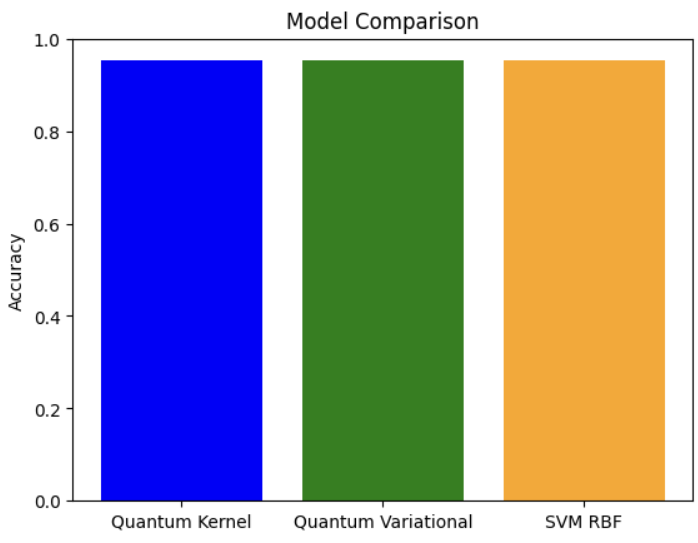
\includegraphics[width=0.5\linewidth]{five.png}
        \caption{Accuracy Comparison}
        \label{fig:enter-label}
    \end{figure}
\end{frame}

\begin{frame}{Model Comparison (Accuracy)}
\begin{block}{Observation}
The bar chart compares the accuracy of three models:
\begin{itemize}
    \item \textcolor{blue}{Quantum Kernel Model (Blue)}
    \item \textcolor{green!60!black}{Quantum Variational Model (Green)}
    \item \textcolor{orange}{SVM with RBF Kernel (Orange)}
\end{itemize}
All models achieve near-perfect accuracy, close to 95\%, indicating that they are effective classifiers for distinguishing fraudulent and non-fraudulent transactions.
Quantum kernel and variational models perform comparably to classical SVM with RBF kernel. This suggests that quantum approaches are capable of exploring complex feature spaces as effectively as traditional methods, paving the way for future quantum advantage in classification tasks.
\end{block}
\end{frame}

\section{Hybrid Quantum Neural Network}
\begin{frame}{Hybrid Quantum Neural Network}
    \begin{itemize}
        \item Neural Network
        \item Drawbacks of Neural Networks
        \item Quantum Neural Network
        \item Why Hybrid Quantum Neural Network?
        \item Data Set Overview
        \item Structures of Neural Networks
        \item Cost Function and Accuracy Comparisons
        \item Why don’t QNN get over-fitted?
        \item Conclusion and Future Works
    \end{itemize}
\end{frame}
\begin{frame}{Neural Networks}
    \begin{figure}
        \centering
        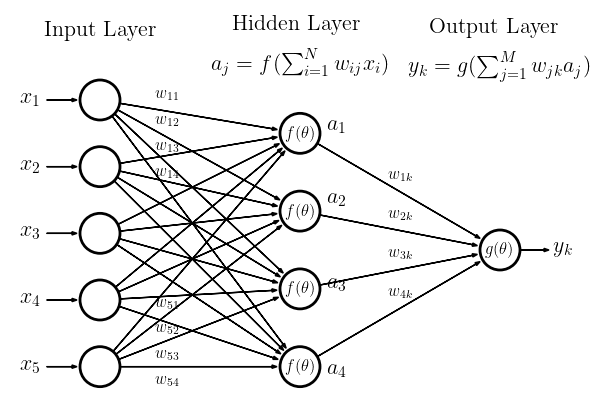
\includegraphics[width=0.7\linewidth]{NN.png}
        \caption{Neural Network}
        \label{fig:enter-label}
    \end{figure}
\end{frame}

\begin{frame}{Drawbacks of Neural Networks}
    \begin{itemize}
        \item \textbf{Require Large Amounts of Data :} Neural networks usually need big datasets to learn effectively, which can be hard to get in some domains.
        \item \textbf{High Computational Cost :} Training and running neural networks often require significant computing power, like GPUs, and can be time-consuming.
        \item \textbf{They Can Overfit Easily :} Neural networks can memorize training data instead of generalizing well, especially if the dataset is small or noisy.
    \end{itemize}
\end{frame}
\begin{frame}{Quantum Neural Network}
    One of the example of Quantum Neural Network is \\
    \textbf{Quantum Orthogonal Neural Network [1] }
    \begin{figure}
        \centering
        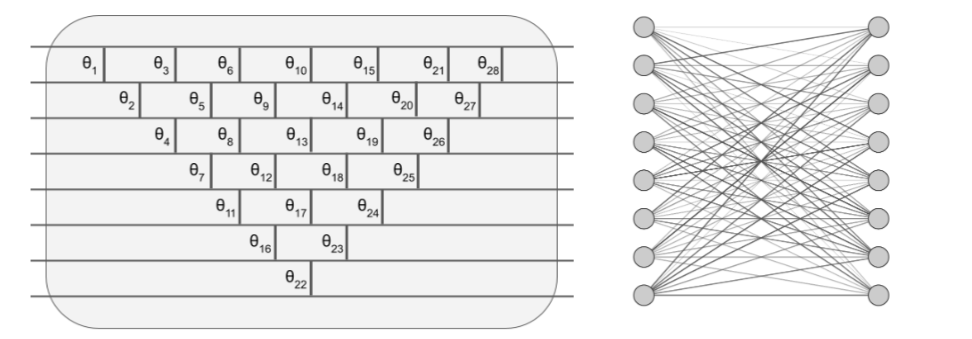
\includegraphics[width=0.5\linewidth]{orthogonal.png}
        \caption{Two equivalent Neural Networks}
        \label{fig:enter-label}
    \end{figure}
    \small [1] Kerenidis, I., Landman, J. and Mathur, N., 2021. Classical and quantum algorithms for orthogonal neural networks. arXiv preprint arXiv:2106.07198.

\end{frame}
\begin{frame}{Why Hybrid Quantum Neural Network?}
    \begin{itemize}
        \item Due to NISQ (Noisy Intermediate Scale Quantum ) Era, the quantum computers have low number of qubits with noisy quantum processing units. For this we can not implement QNN for datasets with a large number of features.  
        \item Reducing dimension or the features of a given dataset by classical methods, we can implement QNN with a capability of complex distributions with high dimensional Hilbert Space.
    \end{itemize}
\end{frame}

\begin{frame}{Data Set Over View}
    
\begin{table}[ht]
\renewcommand{\arraystretch}{0.8}
\centering
\begin{tabular}{|l|l|}
\hline
\textbf{Dataset} & MNIST (Modified NIST) \\
\hline
\textbf{Task} & Binary Classification (Digit \textbf{5} vs \textbf{6}) \\
\hline
\textbf{Total Samples} & $\sim$11,000 images (approx.) \\
\hline
\textbf{Class Labels} & 0 $\rightarrow$ Digit 5 \quad | \quad 1 $\rightarrow$ Digit 6 \\
\hline
\textbf{Training Samples} & $\sim$800 images \\
\hline
\textbf{Test Samples} & $\sim$200 images \\
\hline
\textbf{Image Size} & 28 $\times$ 28 pixels (grayscale) \\
\hline
\vspace{1em}
\textbf{Data Format} & 784-dimensional vectors or 28$\times$28 arrays \\
\hline
\end{tabular}
\end{table}
\begin{figure}
    \centering
    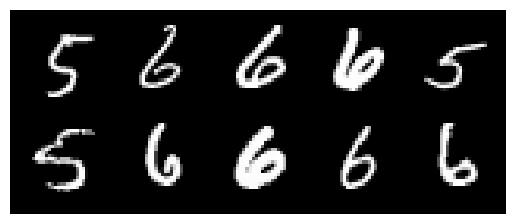
\includegraphics[width=0.4\linewidth]{num.png}
\end{figure}


\end{frame}
\begin{frame}{Structures of Neural Networks}
    \begin{figure}
        \centering
        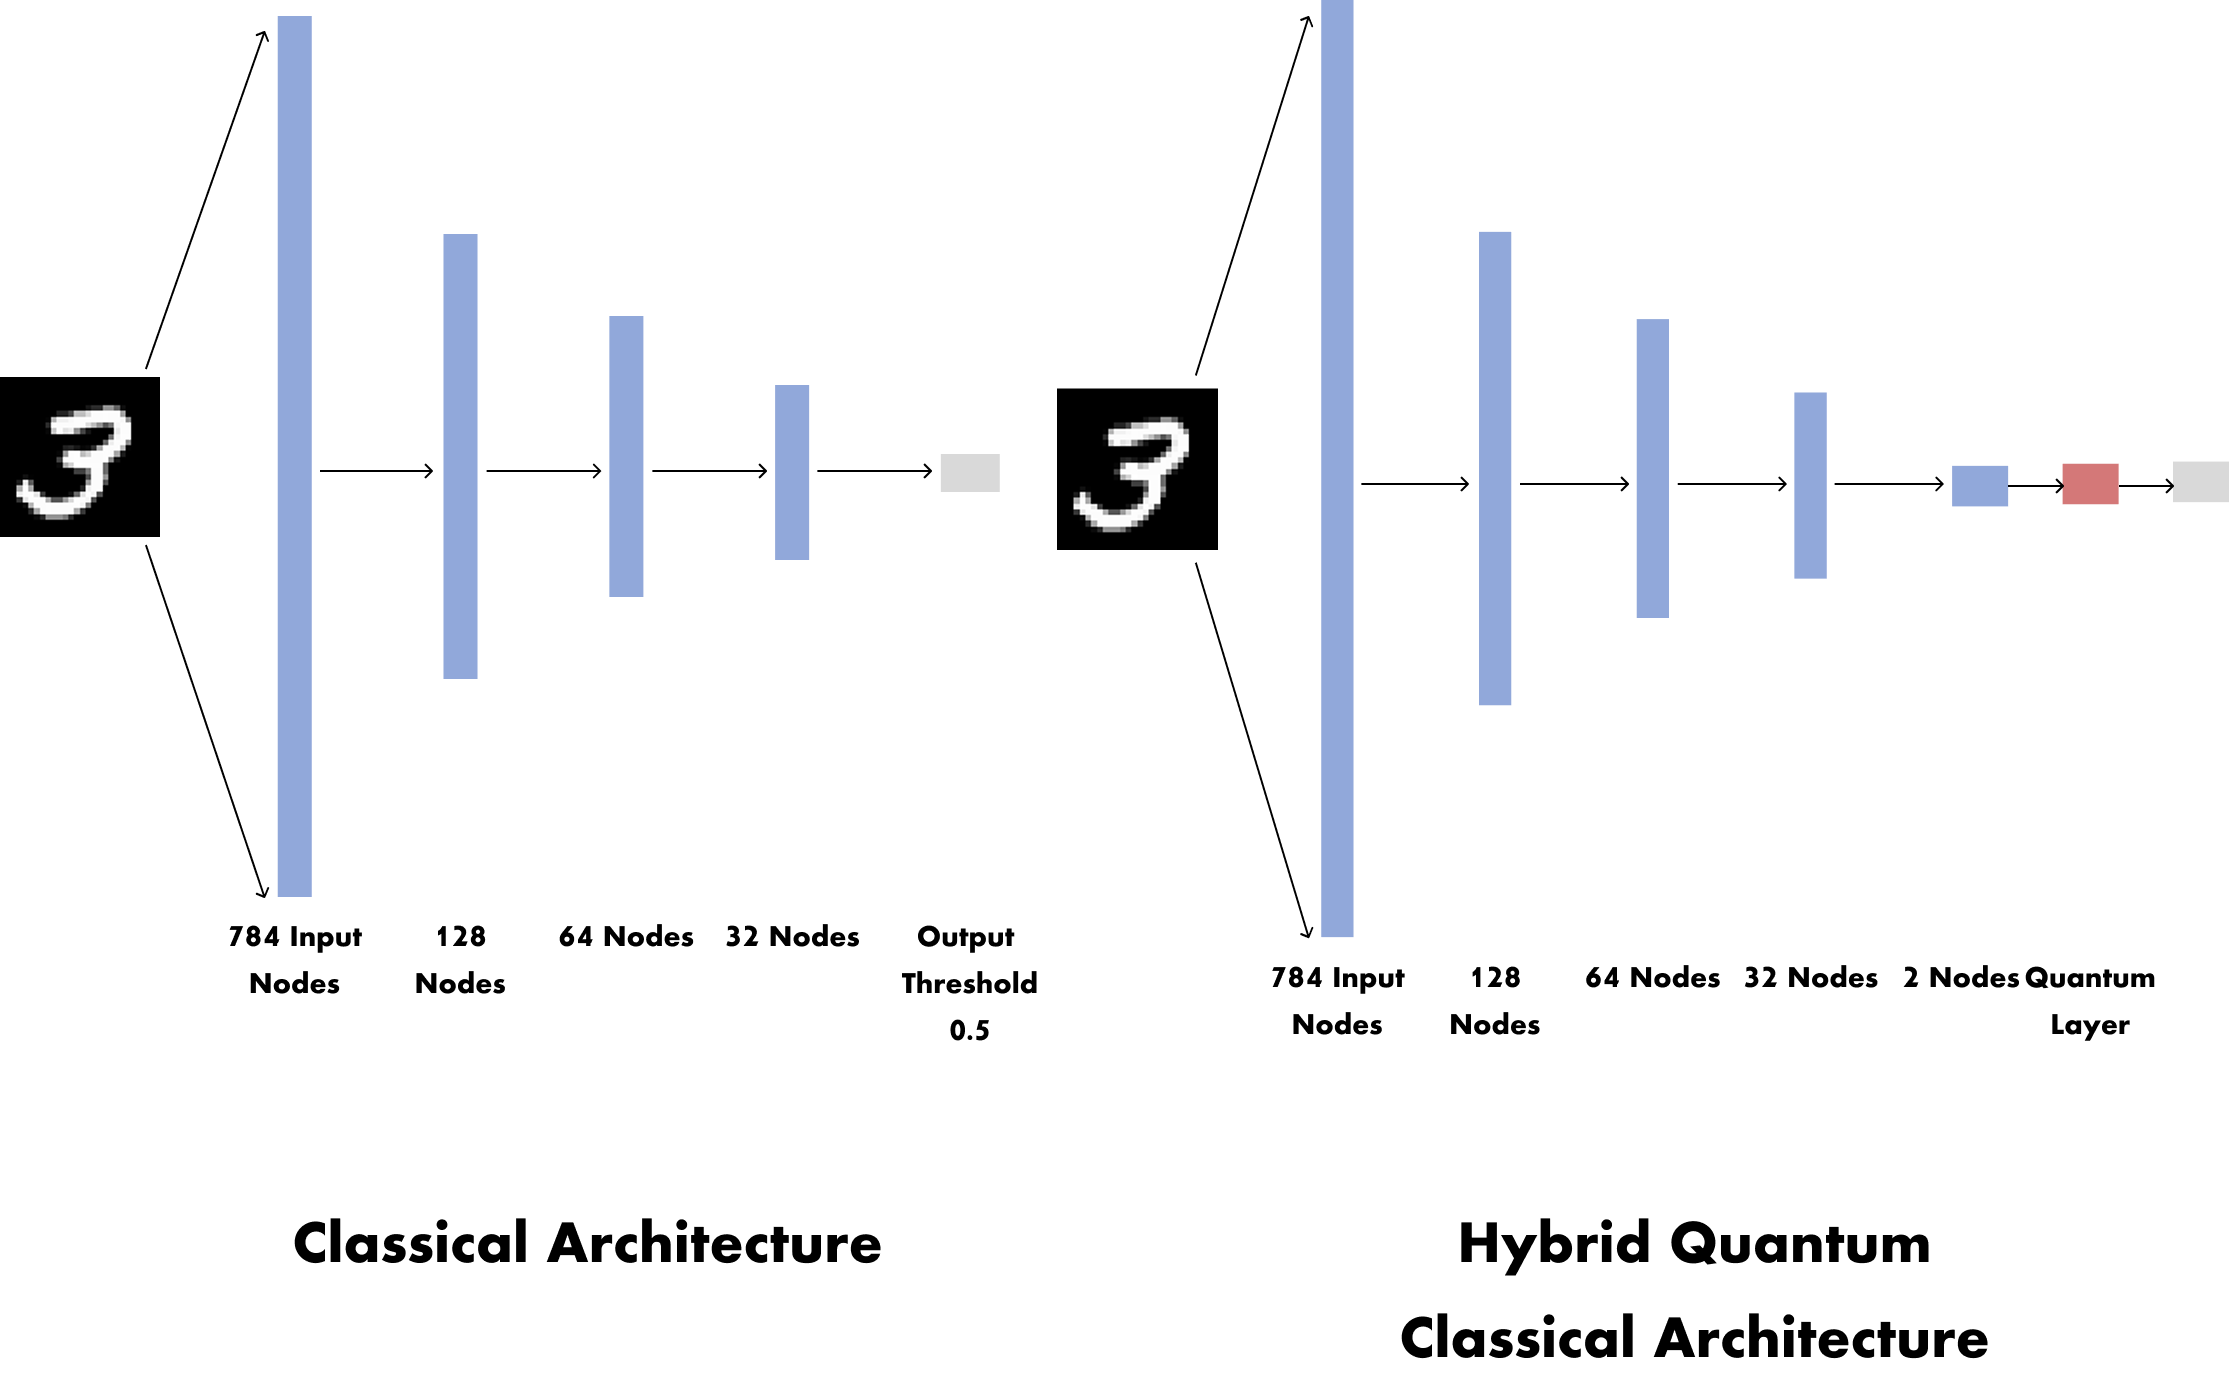
\includegraphics[width=0.6\linewidth]{compari__arch.png}
    \end{figure}
\end{frame}

\begin{frame}{Cost Function and Accuracy Comparisons}
    \begin{figure}
        \centering
        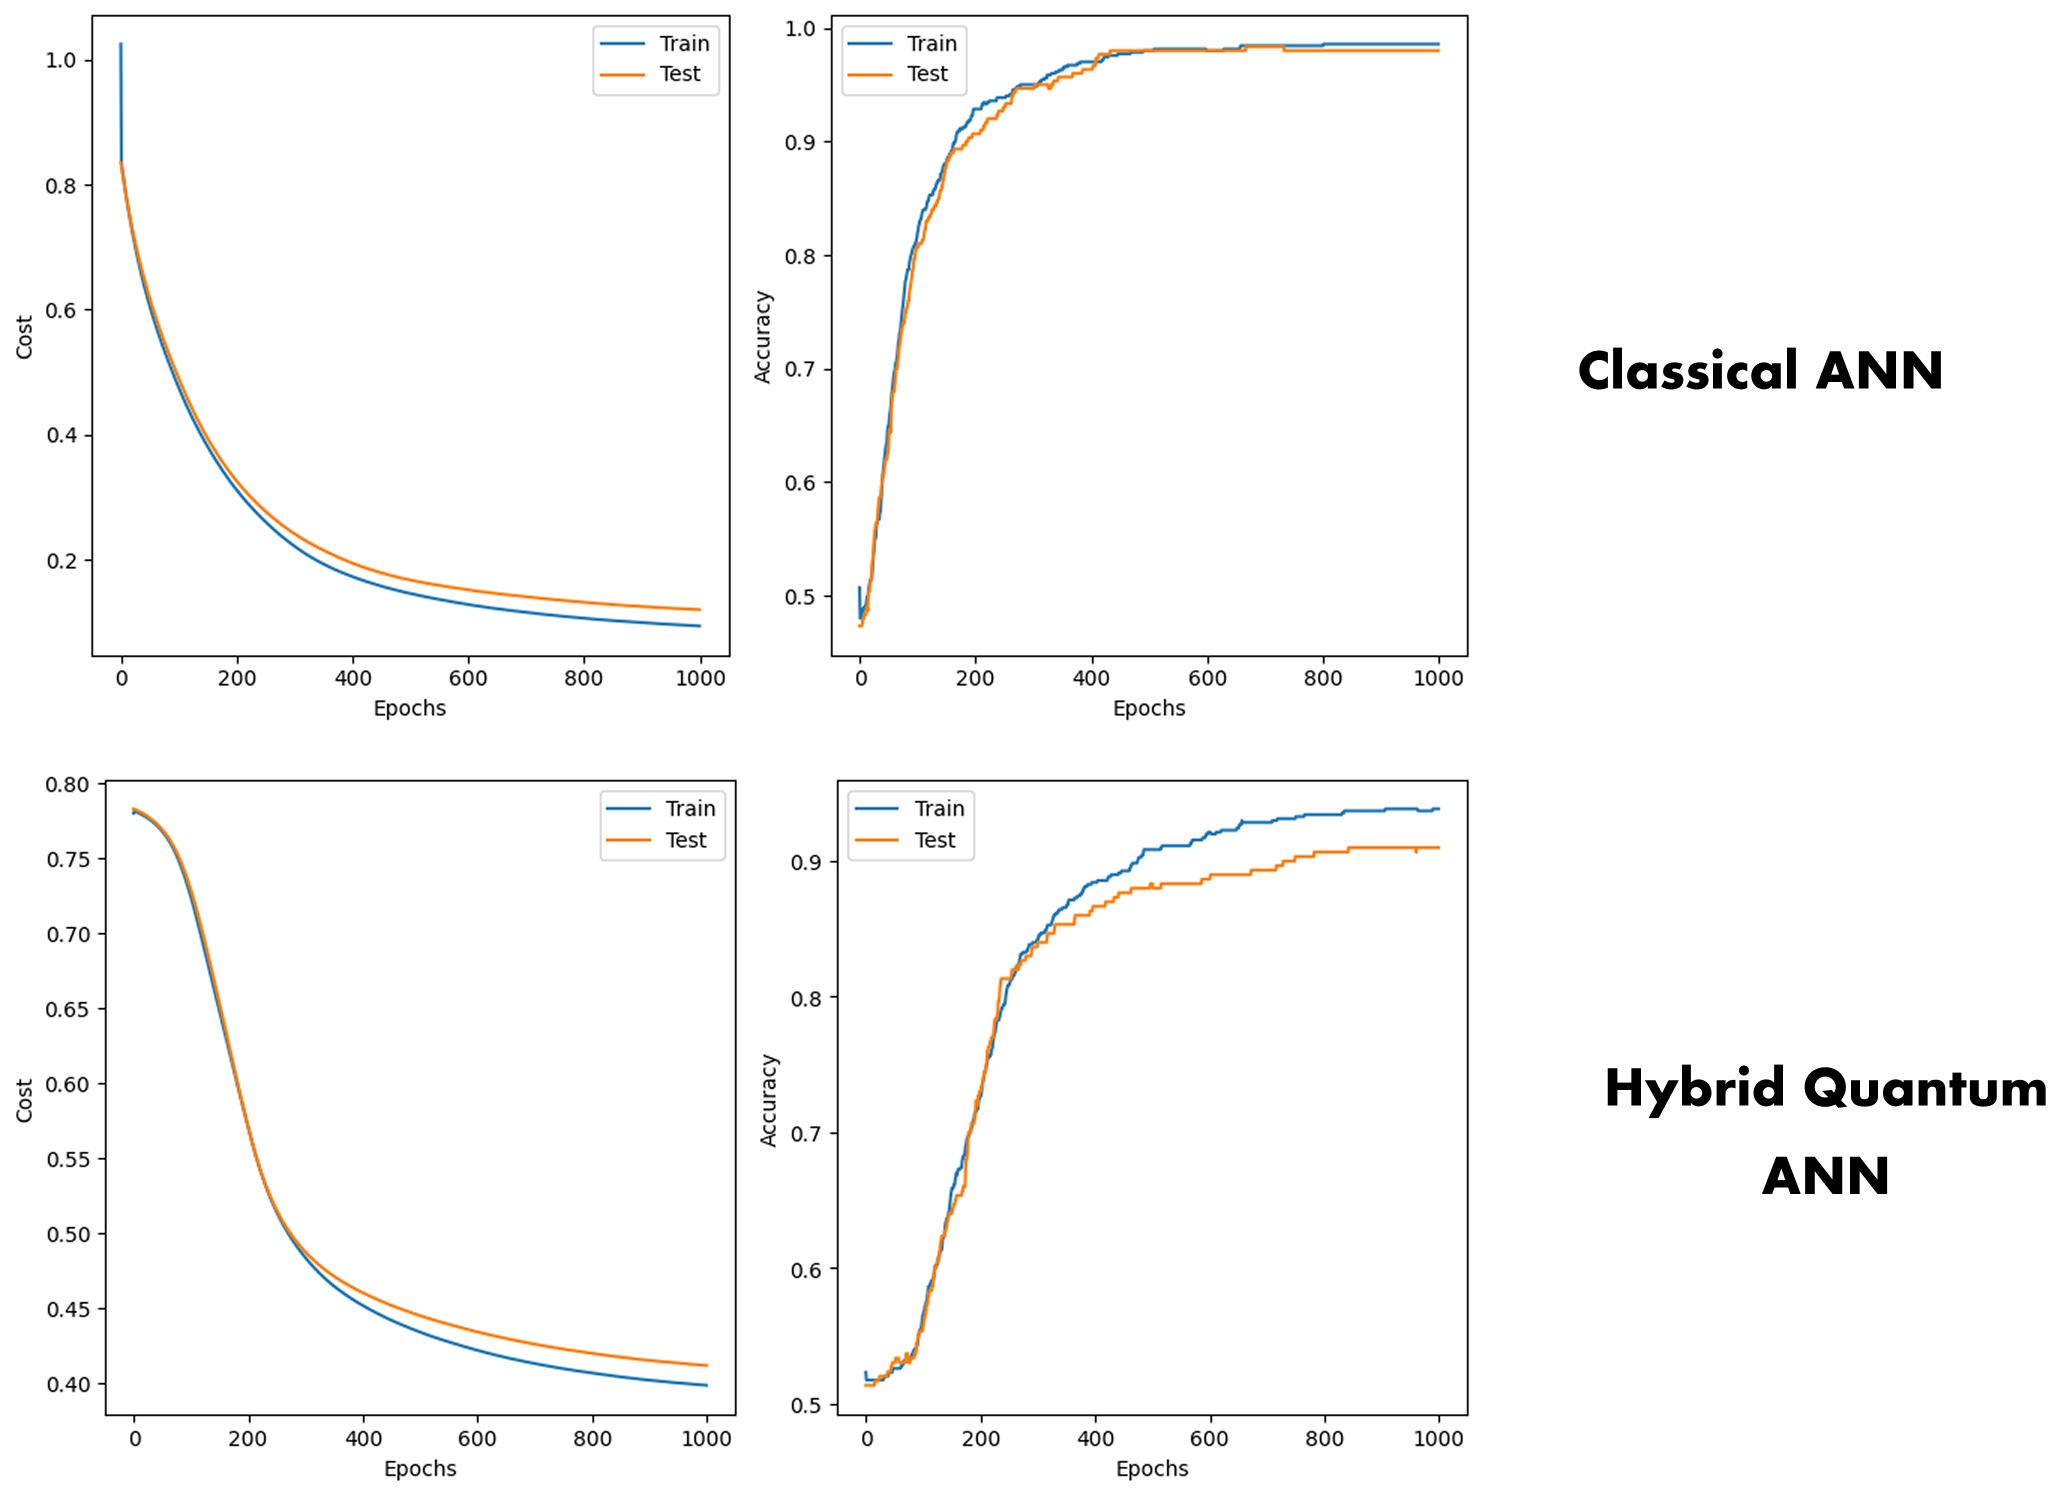
\includegraphics[width=0.6\linewidth]{COMP.png}
    \end{figure}
\end{frame}

\begin{frame}{Why don't QNN get over-fitted?}
    \begin{itemize}
        \item Natural Regularization via Unitarity: Unitary constraints in quantum circuits limit expressivity, preventing overfitting to complex patterns or noise.
        \item Fewer Trainable Parameters: QNNs have smaller parameter spaces, reducing model capacity and overfitting risk.
        \item Smooth Feature Embeddings:  Quantum feature maps highlight global structure and suppress noise, aiding generalization.
    \end{itemize}
\end{frame}
\begin{frame}{Future Works}
    \begin{itemize}
        \item Implement Quantum Convolutional Neural Networks (QCNNs) for improved spatial feature extraction.
        \item Develop a stable solution for multispectral image processing using quantum models.
        \item Establish a mathematical foundation to analyze the relationship between quantum noise and model error.
    \end{itemize}
\end{frame}

\section{Conclusion}
\begin{frame}{Conclusion}
\begin{block}{Overview}
A comparative study of classical SVM and Quantum SVM revealed subtle differences in computational trends and practical applicability, particularly in high-dimensional data classification tasks.
\end{block}

\begin{block}{Quantum Neural Networks vs. Classical Neural Networks}
The comparison between Quantum Neural Networks (QNNs) and traditional neural networks underscores both the promise and limitations of quantum frameworks. While QNNs show potential to outperform classical models in specific contexts, classical neural networks currently maintain a significant edge in scalability and training efficiency—largely due to hardware maturity.
\end{block}

\end{frame}
\begin{frame}{Conclusion}
    \begin{figure}
        \centering
        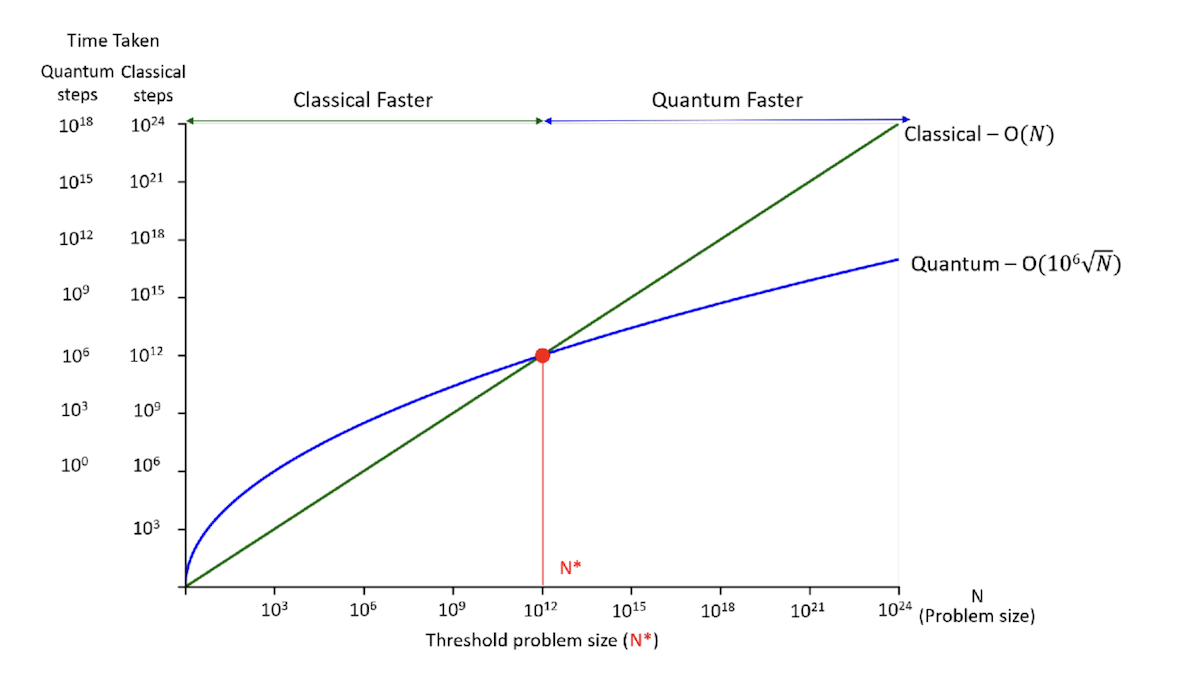
\includegraphics[width=0.6\linewidth]{com.png}
        \caption{Comparing classical and quantum algorithms for text search}
        \label{fig:enter-label}
    \end{figure}
\end{frame}    
\begin{frame}{Conclusion}
\begin{block}{Scalability Insight}
The graph in Figure 33 highlights a crucial characteristic: \textbf{the larger the problem size}, the \textbf{greater the advantage} from using a quantum algorithm. For problems where quantum algorithms offer an improvement, there exists a critical threshold \(N^*\) beyond which quantum speedup surpasses classical performance.

In the case of Grover’s algorithm, the threshold is approximately \(N = 10^{12}\). This means:
\begin{itemize}
    \item Quantum advantage becomes practical only for problems of size at least one trillion.
    \item Quantum computers must handle problems at this scale to be realistically competitive with classical counterparts.
\end{itemize}
\end{block}
\end{frame}
\begin{frame}[plain]
    \centering
    \vspace{2cm}
    {\Huge \textbf{Thank You!}}\\[1.5cm]
    {\large We welcome your questions and feedback}\\[1cm]
    \rule{0.5\linewidth}{0.4pt}\\[1cm]
    \textit{Presented by: Nishanka Das \& Debanjan Kola}\\
    \textit{Institution: Ramakrishna Mission Vivekananda Centenary College}
\end{frame}

\end{document}